\documentclass[12pt,a4paper]{article}
\usepackage[utf8]{inputenc}
\usepackage[french]{babel}
\usepackage[T1]{fontenc}
\usepackage{amsmath}
\usepackage{amsfonts}
\usepackage{amssymb}
\usepackage{graphicx}
\usepackage[left=2cm,right=2cm,top=2cm,bottom=2cm]{geometry}
\usepackage[thinspace,thinqspace,amssymb]{SIunits}
\usepackage{eurosym}

\usepackage{hyperref}
\hypersetup{
    colorlinks=true,
    urlcolor=theme
}

\title{Mise en perspective didactique d'un dossier de recherche}
\author{\textbf{Rémi Metzdorff}}
%\date{Concours externe spécial de l'agrégation de physique-chimie option physique }
\date{2020}

\renewcommand{\d}{\mathrm{d}}
\newcommand{\uroc}{\micro RoC}

%%%%%%%%%%%%%%%%%%%%%%%%%%%%%%  For CV  %%%%%%%%%%%%%%%%%%%%%%%%%%%%%%
\usepackage{array}
%\newcolumntype{L}[1]{>{\raggedright\let\newline\\\arraybackslash\hspace{0pt}}m{#1}}
%\newcolumntype{C}[1]{>{\centering\let\newline\\\arraybackslash\hspace{0pt}}m{#1}}
%\newcolumntype{R}[1]{>{\raggedleft\let\newline\\\arraybackslash\hspace{0pt}}m{#1}}
%%%%%%%%%%%%%%%%%%%%%%%%%%%%%%%%%%%%%%%%%%%%%%%%%%%%%%%%%%%%%%%%%%%%%%

\usepackage{xcolor}
\definecolor{theme}{RGB}{56,115,179}
\usepackage[font=small]{caption}

%%%%%%%%%%%%%%%%%%%%%%%%%%%%%%%%%%%%%%%%%%%%%%%%%%%%%%%%%%%%%%%%%%%%%%
\usepackage[framemethod=tikz]{mdframed}

\mdfdefinestyle{s_mep}{
	linecolor=theme!,
	outerlinewidth=3pt,
	frametitlerule=false,
	topline=false,
	bottomline=false,
	rightline=false,
	backgroundcolor=white,
	innertopmargin=5pt,
	roundcorner=0pt,
	%skipabove=5pt,
	skipbelow=5pt
}
\newmdenv[style=s_mep]{mep_env}

\newenvironment{mep}{%\stepcounter{exa}%
%\newenvironment{myenv}{\begin{adjustwidth}{2cm}{}}{\end{adjustwidth}}
\addcontentsline{ldf}{figure}{0}%
\begin{mep_env}
\small}
{\end{mep_env}}
%%%%%%%%%%%%%%%%%%%%%%%%%%%%%%%%%%%%%%%%%%%%%%%%%%%%%%%%%%%%%%%%%%%%%%

%\footnote{Abbott \textit{et al.}, Observation of Gravitational Waves from a Binary Black Hole Merger, \textit{Phys. Rev. Lett.} \textbf{116}, (2016)}

%\vspace*{20pt}
%\begin{center}
%\begin{large}
%\textsc{Mise en perspective didactique d'un dossier de recherche}
%\end{large}
%\vspace{10pt}
%Concours externe spécial de l'agrégation de physique-chimie, option physique -- 2020
%\vspace{20pt}
%\textbf{Rémi Metzdorff}
%\end{center}

\begin{document}

\maketitle
%\tableofcontents

\section{Parcours universitaire et scientifique}

\noindent
\begin{tabular*}{\textwidth}{p{0.12\textwidth}<{\raggedleft}p{0.83\textwidth}}
\textcolor{theme}{\rule{0.12\textwidth}{2.5mm}} &
\large\textcolor{theme}{Formation et doctorat} \vspace{3pt} \\
2019--2020 &
\textbf{Préparation à l'agrégation} au centre de l'\'Ecole Normale Supérieure (Montrouge).\\
2015--2019 &
\textbf{Doctorat :} Thèse en optomécanique réalisée au sein de l'équipe \og optomécanique et mesures quantiques \fg{} du laboratoire Kastler-Brossel (LKB, Paris) sous la direction de Pierre-François Cohadon, intitulée \textit{Refroidissement de résonateurs macroscopiques proche de leur état quantique fondamental}, soutenue le 23 juillet 2019. \\
2014--2015 &
\textbf{Master 2 :} Parcours LuMI (Lumière, matière, interactions) du master OMP (Optique, matière, plasma) de l'université Pierre et Marie Curie (UPMC, Paris).
Stage de recherche au LKB avec Pierre-François Cohadon (6 mois) sur l'étude des pertes dans des cavités Fabry-Perot de grande finesse. \\
2013--2014 &
\textbf{Master 1 :} Parcours physique générale du master Physique et applications de l'UPMC (Paris).
Stage au LKB avec Pierre Cladé (4 mois) sur le développement de collimateurs compacts pour les faisceaux d'un piège magnéto-optique sur une expérience de métrologie. \\
2012--2013 &
\textbf{Licence 3 :} Parcours physique-chimie de l'UPMC (Paris). \\
2010--2012 &
\textbf{CPGE :} PCSI et PC$^*$ au lycée Louis-le-Grand (Paris). \vspace{10pt} \\

\textcolor{theme}{\rule{0.12\textwidth}{2.5mm}} &
\large\textcolor{theme}{Enseignements, diffusion et vulgarisation} \vspace{3pt} \\
2015--2018 & \textbf{Missions d'enseignement :} ($\unit{64}{h\per an}$)
\begin{itemize}
\item travaux pratiques d'électromagnétisme (L1) ;
\item travaux dirigés et travaux pratiques de physique expérimentale (L2-L3) : programmation, électronique, Arduino ;
\item travaux pratiques d'optique (M1) : laser, diode laser.
\end{itemize}\\
\vspace{-8mm} 2015--2019 &
\vspace{-8mm}\textbf{Vulgarisation :}
\begin{itemize}
\item \textbf{Un chercheur, Une manip (2019) :} présentations au Palais de la découverte autour de la découverte des ondes gravitationnelles ;
\item \textbf{Olympiades de physique (2017) :} conférence sur la découverte des ondes gravitationnelles devant les candidats.
\item \textbf{E=M6 (2017) :} casser un verre avec la voix, recherche et mise en place de l'expérience, présentation lors du tournage ;
\item \textbf{Fête de la science (2015--2018):} conférence sur la détection d'ondes gravitationnelles, animations et présentation du LKB au grand public, notamment à travers des visites et quelques expériences : résonance optique du sodium, interférence en comptage de photons, etc.
\end{itemize}
\end{tabular*}

\section{Refroidissement vers l'état quantique fondamental}

\subsection{Mesure de déplacements et optomécanique}
\label{sec:intro}

\subsubsection{Les mesures de déplacements et leurs applications}

Les mesures de déplacements sont les mesures les plus précises réalisées à ce jour.
À l'échelle astronomique, on souhaite par exemple connaître la distance (et la vitesse) séparant plusieurs objets afin de déterminer la vitesse d'expansion de l'univers.
À l'échelle microscopique, ces mesures permettent d'élaborer des capteurs variés, très sensibles mais de dimensions très faibles : accéléromètres et gyroscopes en mesurant le déplacement d'une masse test, microscope à force atomique en observant la déviation d'un micro-levier à proximité de la surface d'un échantillon, etc.
De nombreuses méthodes permettent d'effectuer ces mesures, avec des sensibilités adaptées aux phénomènes observés : mesure du flux lumineux reçu d'étoiles au rayonnement connu (étoiles céphéides), à l'aide d'un étalon pour les mesures macroscopiques, capacitives, etc.
 
De nombreux dispositifs de mesure de déplacements utilisent les propriétés remarquables de la lumière.
La \textit{mesure absolue} de la distance Terre-Lune découle par exemple de la détermination du temps de vol d'impulsions lumineuses avec des incertitudes relatives de l'ordre de $10^{-9}$.
Le développement de techniques interferométriques autorise par ailleurs les \textit{mesures relatives} les plus sensibles réalisées à ce jour (Fig.~\ref{fig:displacement_measurement}).

Un des succès majeurs de l'interférométrie optique est la détection des ondes gravitationnelles par les interféromètres des projets Virgo (Cascina, Italie) et LIGO (Hanford et Livingston, États-Unis).
Les développements considérables des dernières décennies ont en effet permis, cent ans après leur prédiction par A. Einstein, l'observation directe d'ondes gravitationnelles issues de la coalescence de deux trous noirs.
\footnote{Abbott \textit{et al.}, Observation of Gravitational Waves from a Binary Black Hole Merger, \textit{Phys. Rev. Lett.}, (2016)}
L'amplitude relative maximale du signal mesuré sur Terre était alors proche de $10^{-21}$, soit un déplacement équivalent mille fois plus petit que la taille d'un proton, ce qui en faisait le signal le plus faible jamais détecté associé à l'évènement le plus violent jamais observé.

Les détecteurs d'onde gravitationnelles sont des interféromètres de Michelson géants dont les bras sont des cavités Fabry-Perot pour augmenter l'effet d'un petit déphasage : la longueur des bras de Virgo est de \unit{3}{\kilo\meter} avec des cavités de finesse 50.
Le passage d'une onde gravitationnelle introduit un déphasage qui peut être mesuré à la sortie de l'appareil comme des variations de l'intensité lumineuse transmise par l'interféromètre.

\subsubsection{L'optomécanique : limite de sensibilité et contrôle de miroirs mobiles}

L'optomécanique est un domaine de recherche qui s'intéresse au couplage entre la lumière et un miroir mobile, initialement développé pour augmenter la sensibilité des mesures interférométriques. 
Dans le cas des interféromètres gravitationnels, toute perturbation du détecteur produit un bruit qui, s'il n'est pas causé par le passage d'une onde gravitationnelle, dégrade la sensibilité de la mesure.
La distribution spectrale de ces bruits dépend de leur nature et leur influence dépend de l'intervalle de fréquences sur lequel est réalisé la mesure.
Par exemple, l'agitation thermique microscopique engendre un mouvement macroscopique de la surface des optiques du détecteur.
C'est le mouvement brownien qu'il est possible de contrôler notamment grâce au choix des matériaux utilisés et de la géométrie des composants.
La réduction des bruits classiques est telle que les bruits quantiques liés au laser lui-même deviennent limitants.

D'une part, le \textit{bruit quantique de phase} influence directement la mesure puisque, contrairement au bruit classique, les fluctuations quantiques de phase sont décorrélées entre les deux bras de l'interféromètre.
D'autre part, le \textit{bruit quantique d'intensité} a deux conséquences : un bruit direct sur l'intensité mesurée à la sortie du détecteur et des fluctuations de la force de pression de radiation qui s'exerce sur les miroirs de l'interféromètre et agit sur leur position.
C'est l'action en retour de la mesure, prédite dès les années 80, qui a contribué à fonder les recherches en optomécanique.
Dans un interféromètre de Michelson, le déplacement $\delta x$ d'un miroir est donc associé à un déphasage
\begin{equation}
\delta \varphi = \delta \varphi ^\mathrm{phase} _\mathrm{q} + \frac{4\pi}{\lambda} ( \delta x + \delta x ^\mathrm{rad} _\mathrm{q} + \delta x_\mathrm{c}),
\label{eq:disp}
\end{equation}
où $\delta \varphi ^\mathrm{phase} _\mathrm{q}$ est le bruit quantique de phase et $\delta x ^\mathrm{rad} _\mathrm{q}$ le bruit de position associé au bruit quantique d'intensité , et où $\delta x_\mathrm{c}$ regroupe les bruits classiques.

\begin{figure}
\center
%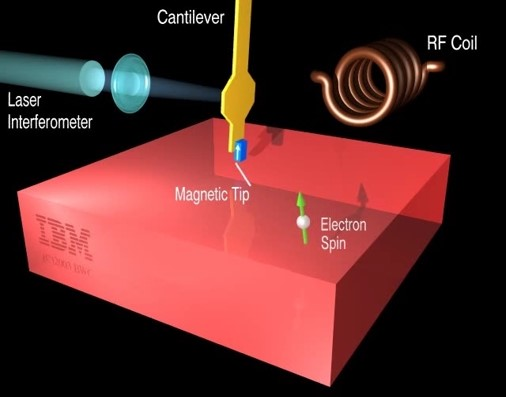
\includegraphics[height=90pt]{figures/AFM_RM.jpg}
%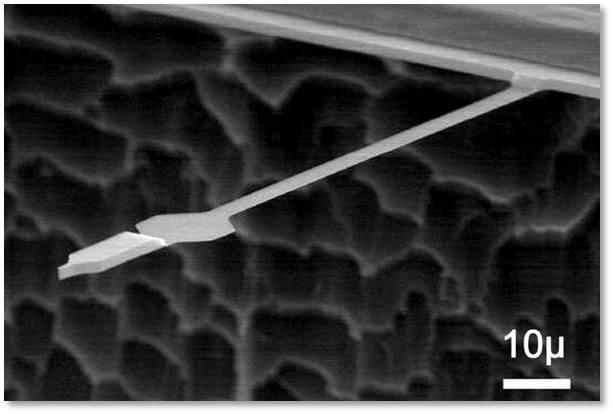
\includegraphics[height=90pt]{figures/AFM_quantilever.png}
%\hfill
%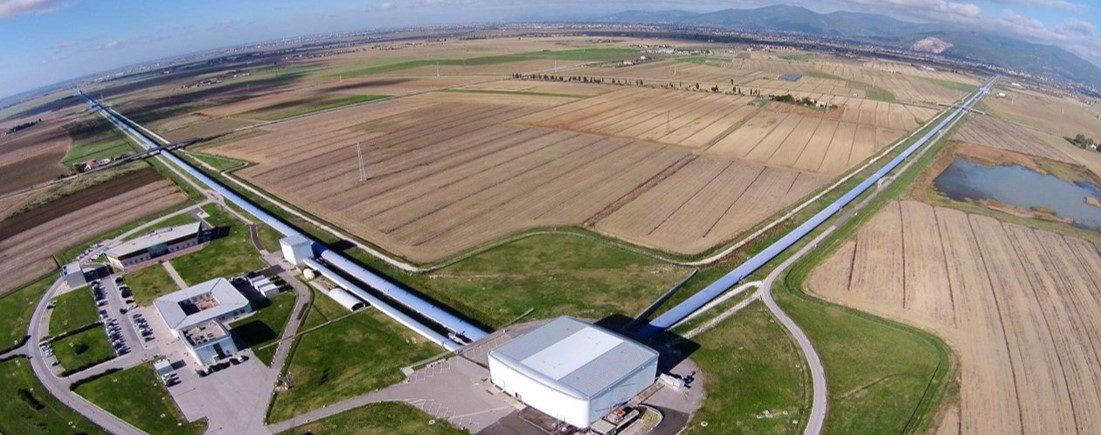
\includegraphics[height=90pt]{figures/virgo.jpg}
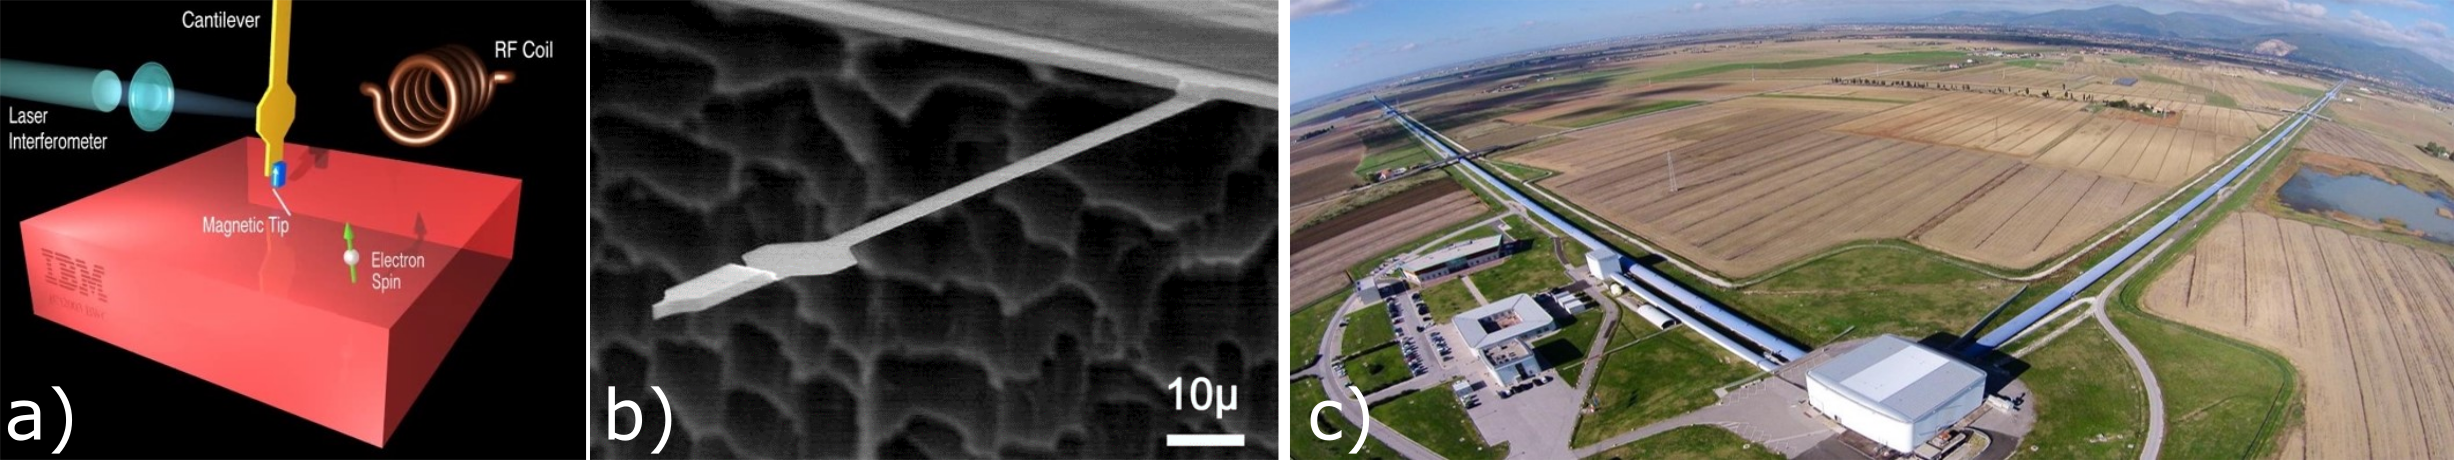
\includegraphics[height=90pt]{figures/displacement.png}
\caption{Les mesures de déplacements sont utiles aussi bien pour sonder la matière que pour des observations astronomiques.
(a) Résonance magnétique par mesure de force (D. Rugar, 2004), capable de détecter des spins uniques exerçant sur (b) le micro-levier une force de l'ordre de $\unit{10^{-18}}{\newton}$, associée à un déplacement de $\unit{10^{-10}}{\meter}$.
(c) Interféromètre gravitationnel Virgo avec ses bras de \unit{3}{\kilo\meter}, qui atteint maintenant une sensibilité relative de l'ordre de $10^{-21}$.}
\label{fig:displacement_measurement}
\end{figure}

L'amplitude du bruit quantique de phase est inversement proportionnelle à l'amplitude du champ lumineux et peut donc être réduite si l'on augmente l'intensité du laser, ce qui justifie les puissances optiques importantes utilisées : $\sim \unit{100}{\kilo\watt}$ dans les cavités.
En revanche, l'amplitude du bruit quantique de pression de radiation est proportionnelle à l'amplitude du champ et est modulée par la réponse mécanique du système.
Pour chaque fréquence de mesure, il existe donc une puissance laser optimale pour laquelle les bruit quantiques de phase et de pression de radiation sont égaux : c'est la \textit{limite quantique standard}.

Même si la pression de radiation peut dégrader la sensibilité des mesures interférométriques, on peut l'exploiter pour contrôler les degrés de liberté mécaniques d'un miroir mobile.
Au cours des vingt dernières années, de nombreux systèmes optomécaniques ont ainsi été développés : capteurs de force, de masse, de température, transducteurs optique-microonde, ponderomotive squeezing, etc.
Une application fondamentale de ces systèmes est l'observation d'effets quantiques sur des objets de plus en plus massifs.

L'objectif de ma thèse est le \textit{refroidissement d'un oscillateur mécanique macroscopique dans son état quantique fondamental}.
Réalisé pour la première fois en 2011 sur un oscillateur de faible masse ($m_\mathrm{eff} = \unit{50}{pg}$) couplé à une cavité microonde\footnote{Teufel \textit{et al.}, Sideband cooling of micromechanical motion to the quantum ground state, \textit{Nature}, (2011)}, l'enjeu repose sur l'utilisation de systèmes de masse effective proche de \unit{100}{\micro\gram}, soit trois ordres de grandeur de plus que les autres expériences actuelles.
Cette masse est choisie proche de la masse de Planck ($m_\mathrm{P}=\unit{22}{\micro\gram}$) au delà de laquelle les effets de décohérence liés à la gravité deviennent significatifs, marquant ainsi la frontière entre les \og mondes \fg{} quantiques et classiques. 
Le système dans son état fondamental permettrai en outre d'\textit{explorer les limites quantiques de sensibilité des mesures de petits déplacements} liées au bruit de pression de radiation, tout en restant beaucoup plus compact que les interféromètres gravitationnels et leurs miroirs ($m_\mathrm{eff}\approx\unit{50}{\kilo\gram}$).
En effet, il est possible d'observer le bruit quantique de pression de radiation pour des puissances optiques modérées une fois un tel refroidissement atteint.

Le refroidissement se fait en utilisant les techniques de l'optomécanique en cavité, pour lesquelles il convient de disposer de \textit{bons} oscillateurs mécaniques : nous les décrirons dans un premier temps.
Pour mesurer leurs déplacements avec précision, ces oscillateurs sont utilisés comme l'un des miroirs d'une cavité optique de grande finesse.
Nous détaillerons ensuite l'utilisation du couplage optomécanique pour le refroidissement de l'oscillateur en cavité.
Le fonctionnement de l'expérience nécessite plusieurs boucles de contrôle qui sont réalisées notamment à l'aide de micro-contrôleurs interfacés en Python.
Nous exposerons finalement les principaux résultats obtenus au cours de la thèse.
Ces résultats seront brièvement mis en perspective dans le cadre de l'amélioration de la sensibilité des détecteurs d'ondes gravitationnelles.

\subsection{Les oscillateurs mécaniques}
\label{sec:mechanical_oscillators}

Bien que leur géométrie soit très variée, le comportement des oscillateurs mécaniques est très bien décrit par un système \{masse, ressort\} amorti soumis à des forces extérieures de résultante $F_\mathrm{ext}$, si bien que l'équation du mouvement s'écrit
\begin{equation}
m_\mathrm{eff}\left[\frac{\d ^2 x(t)}{\d t^2} + \Gamma_m \frac{\d  x(t)}{\d t} +  \Omega_m^2 x(t)\right] = F_\mathrm{ext}(t),
\label{eq:eq_of_motion}
\end{equation}
où $m_\mathrm{eff}$ est la masse effective, $\Omega_m$ la pulsation propre et $\Gamma_m$ l'amortissement.
Le comportement fréquentiel se déduit dans l'espace de Fourier de la susceptibilité mécanique $\chi[\Omega]$ de l'oscillateur :
\begin{equation}
\chi[\Omega] = \frac{1}{m_\mathrm{eff}[(\Omega_m^2-\Omega^2)-i\Gamma_m\Omega]}.
\end{equation}

L'agitation thermique microscopique se traduit au niveau macroscopique comme une excitation du mode propre de l'oscillateur à l'origine du mouvement brownien.
Ces perturbations sont décrites par la théorie de Langevin, où le terme de dissipation $\Gamma_m$ est responsable d'un couplage de l'oscillateur à son environnement assimilé à un bain thermique à la température $T_\mathrm{env}$.
Il en résulte une force fluctuante $F_\mathrm{T}[\Omega]$ dont le spectre est lié à la partie imaginaire de la susceptibilité mécanique par le théorème de fluctuation-dissipation.

Dans le cas où la dissipation est faible ($\Gamma_m \ll \Omega_m$), on montre que le spectre de déplacement de l'oscillateur à l'équilibre thermodynamique avec son environnement est bien décrit par une lorentzienne centrée sur la fréquence propre mécanique, dont l'intégrale (l'aire sous la courbe) est fonction directe du rapport $T_\mathrm{env}/m_\mathrm{eff}$.
Connaissant sa masse effective, \textit{une acquisition du spectre du mouvement brownien de l'oscillateur permet donc de mesurer} $T_\mathrm{env}$ et inversement. 
Le spectre est d'autant plus piqué autour de $\Omega_m$ que la dissipation est faible : on utilise donc des oscillateurs avec des facteurs de qualité mécaniques $Q=\Omega_m/\Gamma_m$ très élevés ($Q>10^6$).

\begin{mep}
En première année de CPGE (PCSI ou MPSI), l'étude des propriétés classiques de ces oscillateurs pourrait être menée lors des cours de mécanique et en particulier de l'étude de l'oscillateur harmonique amorti en régime libre ou forcé.
L'évolution de l'amortissement peut être reliée à la viscosité du fluide dans lequel est plongé l'oscillateur, celle de la fréquence reliée à la masse effective pour obtenir une balance, etc.
Ceci fournit plusieurs exemples pratiques d'utilisation de tels objets comme capteurs notamment, qu'il est possible d'exploiter en TP.
La description fréquentielle de la réponse mécanique me semble également pertinente pour faire comprendre aux étudiants la notion de filtrage et pourrait ainsi être rapprochée de l'étude des filtres électroniques.
\end{mep}

Cette description classique ne permet cependant pas d'expliquer le comportement de l'oscillateur aux très basses températures.
Il est nécessaire d'utiliser un modèle quantique, où le hamiltonien du système est celui d'une masse $m_\mathrm{eff}$ dans un puits de potentiel de pulsation $\Omega_m$ à une dimension.
La résolution de l'équation de Schrödinger conduit à une quantification des niveaux d'énergie $E_n = \hbar\Omega_m (n_\mathrm{T}+\frac{1}{2})$, où $n_\mathrm{T}$ est le nombre de phonons qui caractérise l'état de l'oscillateur.
Le niveau d'occupation du système est alors donné par la statistique de Bose-Einstein :
\begin{equation}
n_\mathrm{T} = \left[ e^\frac{T_Q}{T} -1\right]^{-1},
\label{eq:phonon_number}
\end{equation}
où la température quantique $T_Q$ est définie par $T_Q = \hbar\Omega_m/k_B$.
En particulier, l'énergie minimale du système dans son état fondamental n'est pas nulle et induit un bruit de position appelé \og fluctuations de point zéro\fg{}.
Il s'agit donc pour nous de refroidir un oscillateur mécanique à une température $T$ pour laquelle $n_\mathrm{T}<1$, c'est à dire $T<T_Q$.

\begin{mep}
Même si l'étude d'une particule dans un puits de potentiel harmonique n'est pas au programme de CPGE, l'étude quantique de ces systèmes pourrait faire l'objet d'une approche documentaire dans laquelle les étudiants seront amenés à effectuer la comparaison avec le cas d'un puits de potentiel de profondeur finie.
En MP, je pourrais aller jusqu'à l'étude statistique permettant de retrouver l'expression~\eqref{eq:phonon_number} pour discuter de l'état du système en fonction de la température.
\end{mep}

\begin{figure}
\center
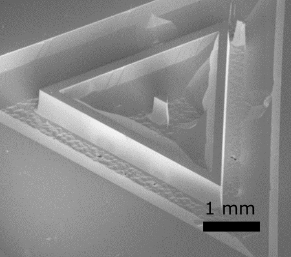
\includegraphics[height=90pt]{figures/micropillar.png}
\hfill
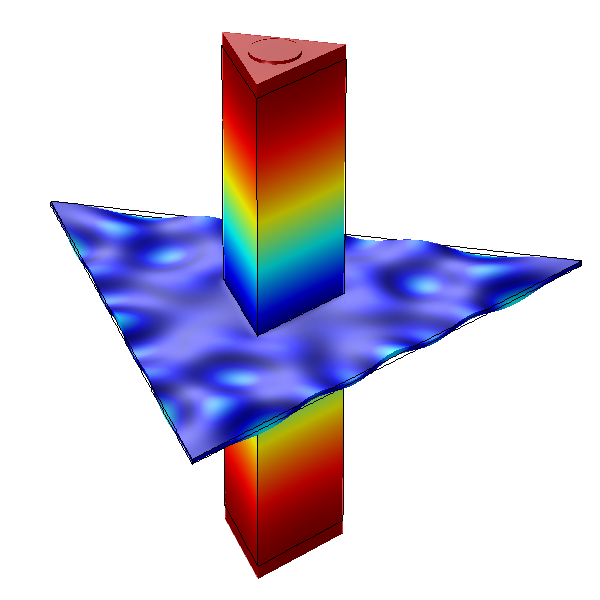
\includegraphics[height=90pt]{figures/micropillar_disp.png}
\hfill
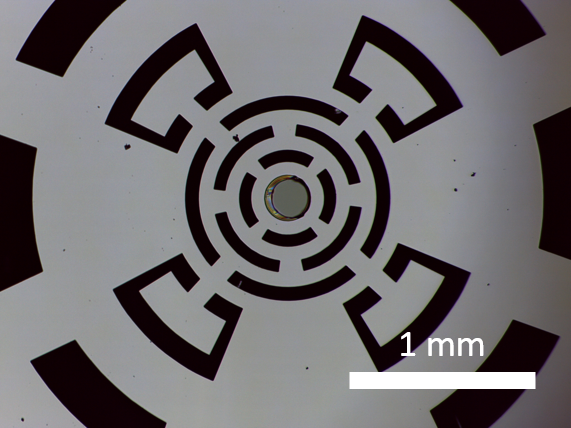
\includegraphics[height=90pt]{figures/microwheel.png}
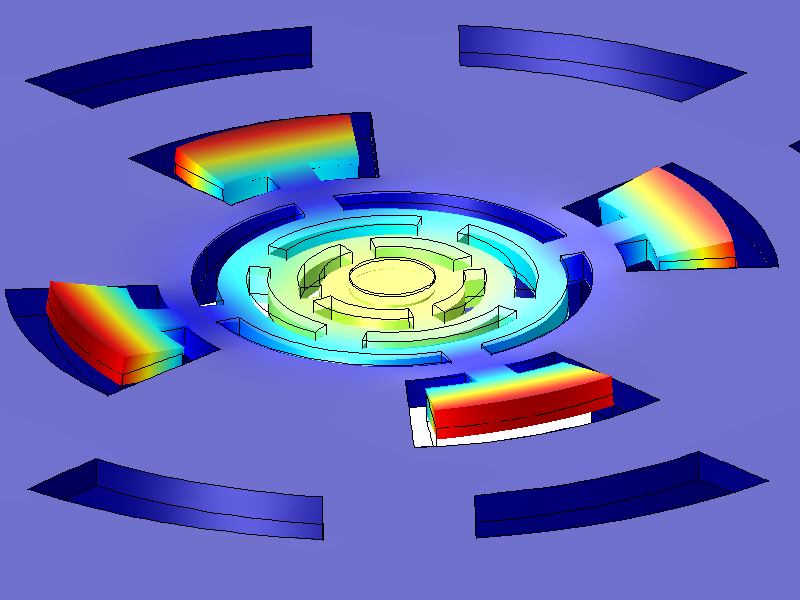
\includegraphics[height=90pt]{figures/microwheel_disp.png}
\caption{À gauche : image obtenue par microscopie électronique d'un micro-pillier et simulation par élément fini (COMSOL) du mode propre de compression utilisé.
À droite : image obtenue par microscopie optique d'un micro-disque et simulation du mode propre utilisé.
Le code couleur correspond au déplacement de la structure, du bleu au rouge, le rouge correspondant au déplacement maximal.}
\label{fig:resonators}
\end{figure}

Au cours de ma thèse, j'ai utilisé deux types d'échantillons (Fig.~\ref{fig:resonators}) :
\begin{itemize}
\item un micro-pilier en quartz de \unit{1}{\milli\meter} de long, de section triangulaire de \unit{240}{\micro\meter} de côté, micro-fabriqué à l'ONERA (Paris).
Il est suspendu en son milieu par une membrane d'environ \unit{10}{\micro\meter} d'épaisseur et on dépose un miroir de très haute réflectivité sur l'une de ses extrémités, en collaboration avec le LMA (Lyon).
Avec $m_\mathrm{eff}=\unit{33{,}5}{\micro\gram}$ et $\Omega_m=2\pi\times\unit{3{,}6}{\mega\hertz}$, on a $T_{Q}^\mathrm{pilier} = \unit{200}{\micro\kelvin}$ avec des facteurs de qualité allant jusqu'à $10^7$ ;
\item un micro-disque en silicium obtenu en collaboration avec l'UniFI (Italie) d'environ $\unit{200}{\micro\meter}$ de diamètre, sur lequel est déposé un miroir de très haute réflectivité.
Avec $m_\mathrm{eff}=\unit{112}{\micro\gram}$ et $\Omega_m=2\pi\times\unit{280}{\kilo\hertz}$, on a $T_{Q,\mathrm{disque}} = \unit{10}{\micro\kelvin}$ avec $Q\approx10^6$.
\end{itemize}
Avant d'être utilisés pour les expériences de refroidissement, les échantillons doivent être caractérisés soigneusement, notamment pour la thermométrie à basse température.
Avec une cale piézoélectrique par exemple, on étalonne tout d'abord leur réponse mécanique à une excitation forcée, ce qui permet d'observer les différents modes mécaniques et de mesurer $\Omega_m$ et $Q$.
\`A température ambiante, la thermalisation est suffisante pour que la température de l'échantillon soit proche de celle que nous donne une simple thermistance située à proximité.
La masse effective des oscillateurs $m_\mathrm{eff}$ est alors obtenue en mesurant leur mouvement brownien par interférométrie optique.
Les paramètres $\Omega_m$ et $Q$ dépendent fortement de la température et de la pression  : l'échantillon est donc placé dans un cryostat à circulation d'hélium permettant d'atteindre rapidement des températures de l'ordre du kelvin et des pressions inférieures à $\unit{10^{-5}}{\milli bar}$.
On voit sur la Fig.~\ref{fig:thermal_noise} que le refroidissement de l'échantillon s'accompagne d'un déplacement de sa fréquence de résonance et d'une augmentation de son facteur de qualité, liés à la dépendance des propriétés mécaniques des matériaux avec la température.
La diminution de l'aire sous le pic proportionnelle à $T_\mathrm{env}$ traduit le mouvement brownien, plus faible à basse température.

\begin{mep}
La plupart des techniques employées pour nos échantillons peuvent être adaptées pour la caractérisation mécanique d'un diapason ou d'un verre vibrant.
Par exemple, en terminale scientifique, je pourrai proposer une approche expérimentale afin de mesurer le facteur de qualité mécanique à partir de la décroissance du son émis par ces objets.
A l'aide de considérations énergétiques, les élèves seraient amenés à discuter des sources de perte qui influent sur le facteur de qualité : frottements, rayonnement d'ondes sonores, etc.
Je pourrai finalement montrer aux élèves comment ces techniques sont utilisées en recherche grâce à une visite du laboratoire.
\end{mep}

\begin{figure}
\center
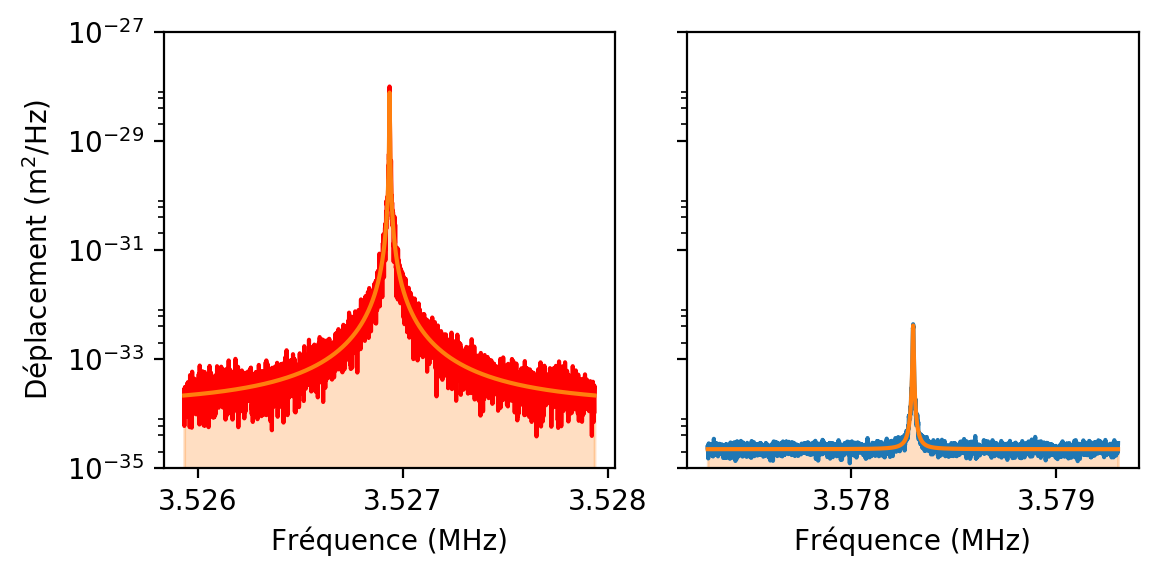
\includegraphics[scale=0.75]{figures/thermal_peak_def_filled.png}
\caption{Spectres des fluctuations de position d'un micro-pilier dues au mouvement brownien de l'oscillateur.
Le déplacement est exprimé en $\meter\squared{.}\hertz^{-1}$ car on s'intéresse non à l'amplitude mais à la densité spectrale de puissance du bruit de position.
La figure de gauche est obtenue à température ambiante ($\sim\unit{300}{\kelvin}$) et celle de droite en cryogénie ($\sim\unit{30}{\milli\kelvin}$).}
\label{fig:thermal_noise}
\end{figure}

\subsection{Une cavité optique pour augmenter la sensibilité}
\label{sec:cavity}

Nous l'avons dit, les déplacements de l'oscillateur sont mesurés par interférométrie optique : un faisceau laser se réfléchit sur un miroir mobile et acquiert un déphasage $\delta\varphi$ qui dépend du déplacement $\delta x$ du miroir.
La sensibilité $\delta\varphi / \delta x$ de la mesure dépend de la détection employée.
Dans le cas d'un interféromètre de Michelson dont l'un des bras porte le miroir mobile, la sensibilité vaut $4\pi/\lambda$ et ne dépend que de la longueur d'onde du laser.
L'utilisation d'une cavité de finesse $\cal{F}$ permet d'amplifier le déphasage : si la cavité est résonante avec le laser, on a
\begin{equation}
\delta \varphi = 8{\cal{F}}\frac{\delta x}{\lambda},
\end{equation}
car la lumière effectue alors en moyenne ${\cal{F}}$ allers-retours dans la cavité.
Le déphasage est ensuite converti en variation d'intensité en faisant interférer ce faisceau signal avec un faisceau de référence, appelé oscillateur local.

Plusieurs détections ont ainsi été implémentées, chacune possédant des avantages et inconvénients quant à la sensibilité et la simplicité de mise en œuvre.
Pour les caractérisations préliminaires des échantillons, un simple interféromètre de Michelson convient puisqu'on étudie un régime forcé (grâce à une cale piézoélectrique) pour lequel l'amplitude des déplacements est grande.
En revanche, pour les mesures de mouvement brownien, la sensibilité de l'interféromètre de Michelson est insuffisante et il est nécessaire d'utiliser une cavité Fabry-Perot dont l'un des miroirs est celui de l'oscillateur mécanique.
On détecte alors la lumière réfléchie par la cavité :
\begin{itemize}
\item détection directe : si la cavité est légèrement désaccordée par rapport au laser, une variation de sa longueur provoqué par un déplacement de l'oscillateur est directement responsable de variations de l'intensité réfléchie ;
\item détection homodyne : si la cavité est résonante avec le laser, aucune variation d'intensité n'est mesurable mais la sensibilité $\delta\varphi/\delta x$ est maximale.
En faisant interférer le faisceau réfléchi par la cavité avec un faisceau de référence dans un interféromètre de Michelson, on observe les variations de l'intensité transmise par l'interféromètre.
L'utilisation d'une détection équilibrée, non représentée ici, permet d'atténuer fortement les bruits classiques, ce qui autorise des mesures limitées par les bruits quantiques. 
\end{itemize}
Le principe de ces détections est présenté en Fig.~\ref{fig:detection_scheme}.
D'autres méthodes (Pound-Drever-Hall, détection synchrone, hétérodyne) sont aussi nécessaires mais elles ne seront pas présentées ici.

\begin{figure}
\center
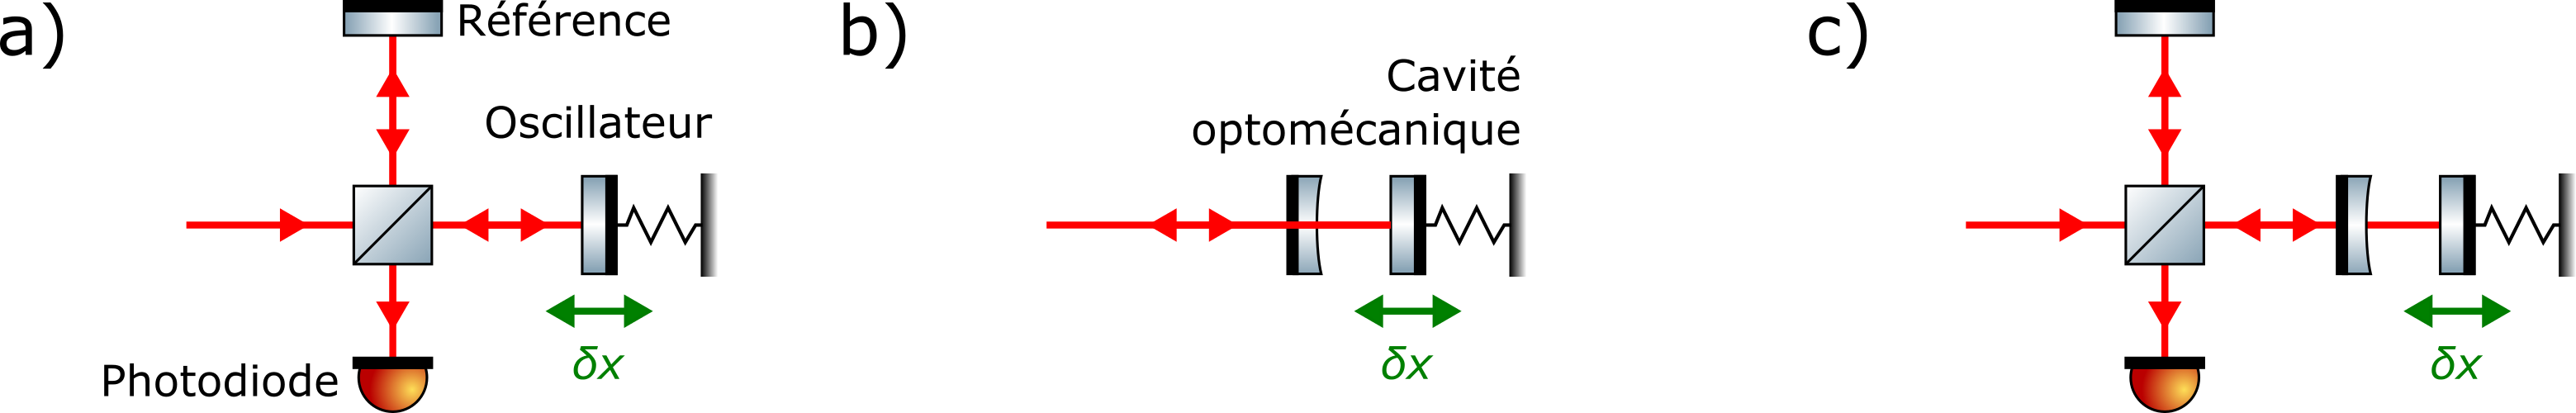
\includegraphics[scale=0.8]{figures/detection_scheme.png}

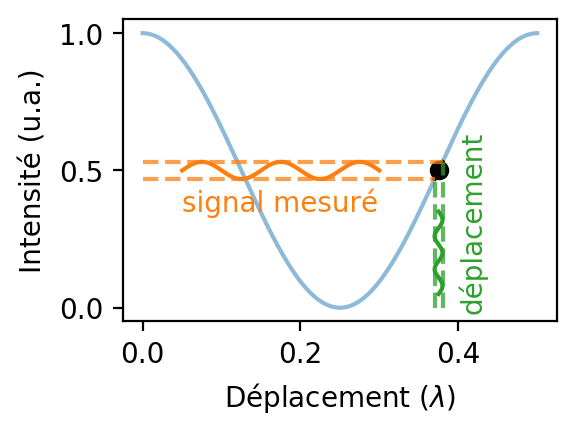
\includegraphics[scale=0.75]{figures/michelson_response.png}
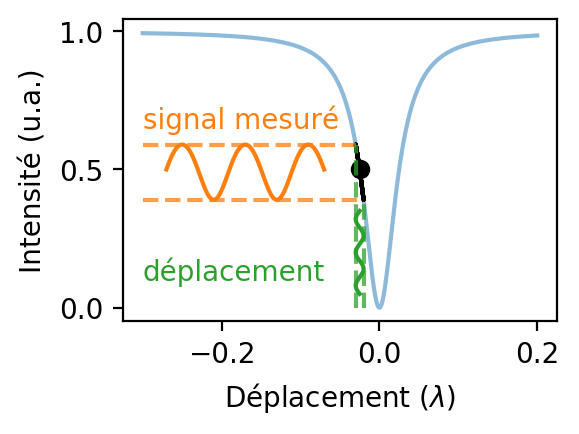
\includegraphics[scale=0.75]{figures/cavity_intensity_response.png}
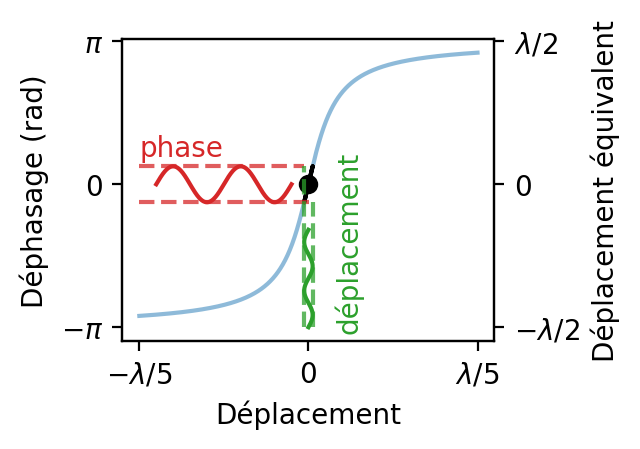
\includegraphics[scale=0.75]{figures/cavity_phase_response.png}
\caption{Schéma simplifié de trois dispositifs utilisés pour la mesure de petits déplacements avec un laser de longueur d'onde $\lambda$.
(a) Mesure de l'intensité transmise par un interféromètre de Michelson, (b) de l'intensité réfléchie par une cavité Fabry-Perot (${\cal{F}}=20$) et (c) de la phase du faisceau réfléchi par la même cavité.
Les graphes indiquent la réponse de la détection (en bleu) en fonction de la position du miroir et l'allure du signal mesuré (en orange) lors d'un petit déplacement $\delta x$ (en vert) au point de fonctionnement optimal (en noir) où la sensibilité est maximale.
Pour le graphe (c), seule la réponse en phase de la cavité est tracée et il faut en plus tenir compte de la réponse de l'interféromètre.}
\label{fig:detection_scheme}
\end{figure}

Compte tenu de la faible dimension des miroirs plans déposés sur les oscillateurs mécaniques, il est nécessaire d'utiliser à l'entrée de la cavité un miroir d'un rayon de courbure de l'ordre du millimètre (\uroc).
Avec un laser $\mathrm{CO_2}$, j'ai fabriqué par photoablation multiple des structures concaves d'environ $\unit{200}{\micro\meter}$ de diamètre, possédant des rayons de courbure variés.
Un dépôt diélectrique de couches de silice $\mathrm{SiO_2}$ et d'oxyde de tantale $\mathrm{Ta_2O_5}$ réalisé au Laboratoire des matériaux avancés (Lyon) permet ensuite d'obtenir des miroirs ayant une transmission bien contrôlée entre 0 et $\unit{120}{ppm}$ pour nos échantillons.
J'ai ensuite réalisé un ensemble de pièces mécaniques en cuivre de haute pureté (Fig.~\ref{fig:cavity}) permettant un assemblage et un alignement rapide d'une cavité de $\unit{100}{\micro\meter}$ de longueur, constituée d'un échantillon (micro-pilier ou micro-disque) et d'un \uroc\ comme miroir d'entrée, qui permet un asservissement de la longueur de cavité sur le laser et compatible avec une utilisation dans un cryostat.

\begin{mep}
Dans le cadre d'un projet expérimental et numérique de l'enseignement scientifique en première, je pourrai proposer aux élèves un interféromètre de Michelson imprimable en 3D.
Cet interféromètre peut être asservi avec un Arduino et une interface Python pour mettre en évidence l'importance du choix du point de fonctionnement sur la sensibilité par exemple.
Ils s'agirait de mettre pratique diverses compétences : impression 3D, programmation, mesures et incertitudes.
En deuxième année de CPGE, je pourrai aussi utiliser de nombreux dispositifs interférentiels pour mettre en évidence l'importance des interférences dans les mesures de précision : interféromètres de Michelson et Mach-Zender, Fabry-Perot.
Certaines méthodes de détections impliquent une modulation/démodulation de l'information (le déplacement) sur une porteuse (le laser) qu'on peut rapprocher des méthodes employées dans les télécommunications avec des étudiants en PSI.
\end{mep}

\begin{figure}
\center
%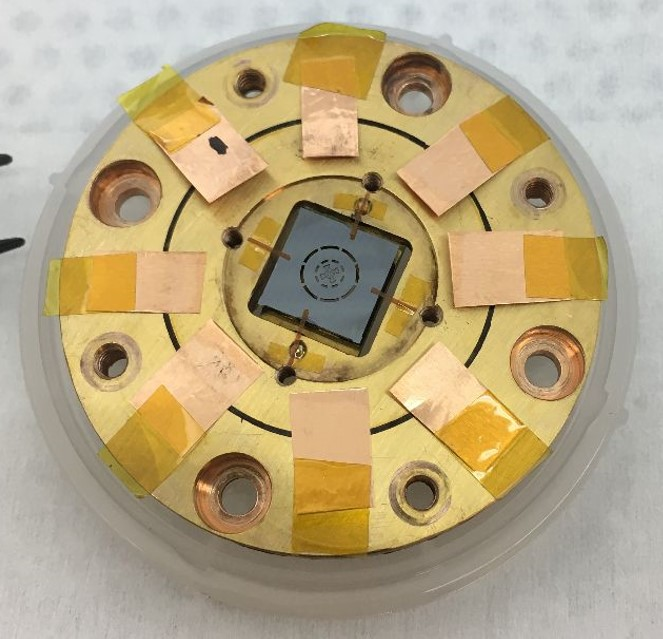
\includegraphics[height=130pt]{figures/cavity_microwheel.jpg}
%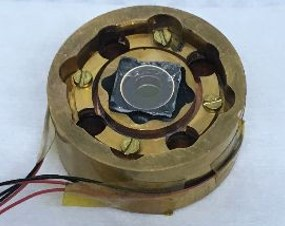
\includegraphics[height=130pt]{figures/cavity_uroc.jpg}
%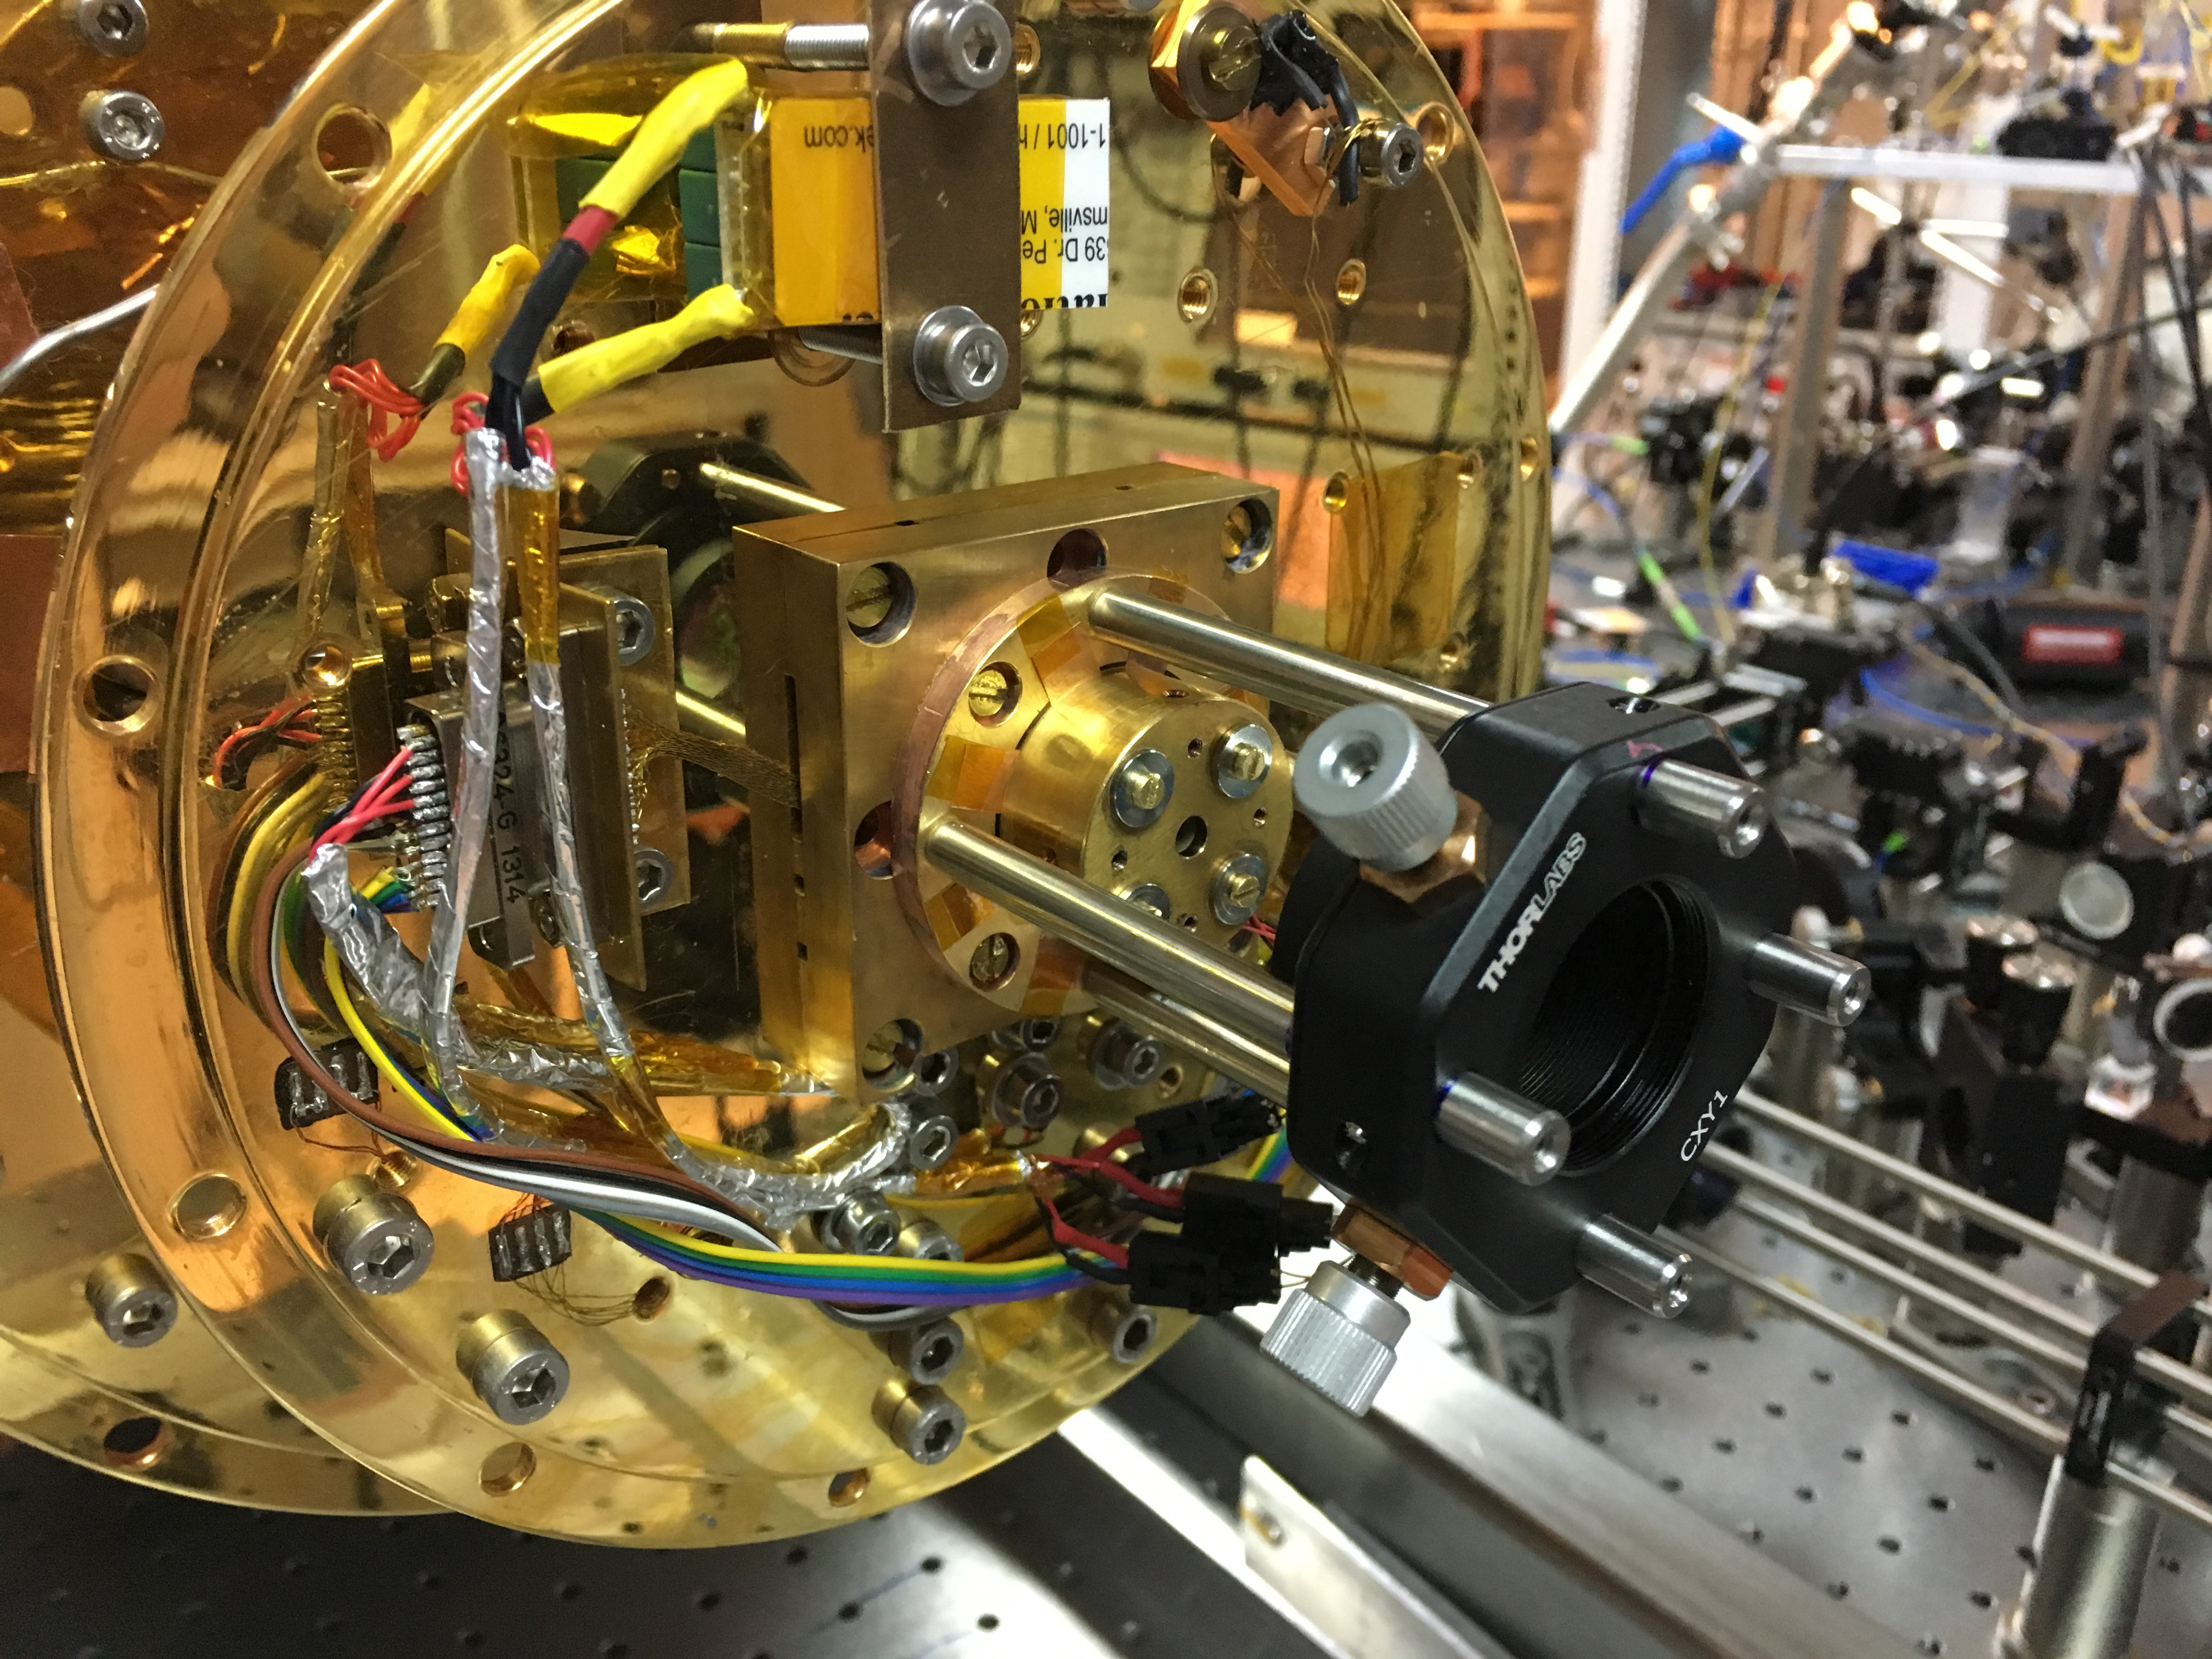
\includegraphics[height=130pt]{figures/IMG_1766.JPG}
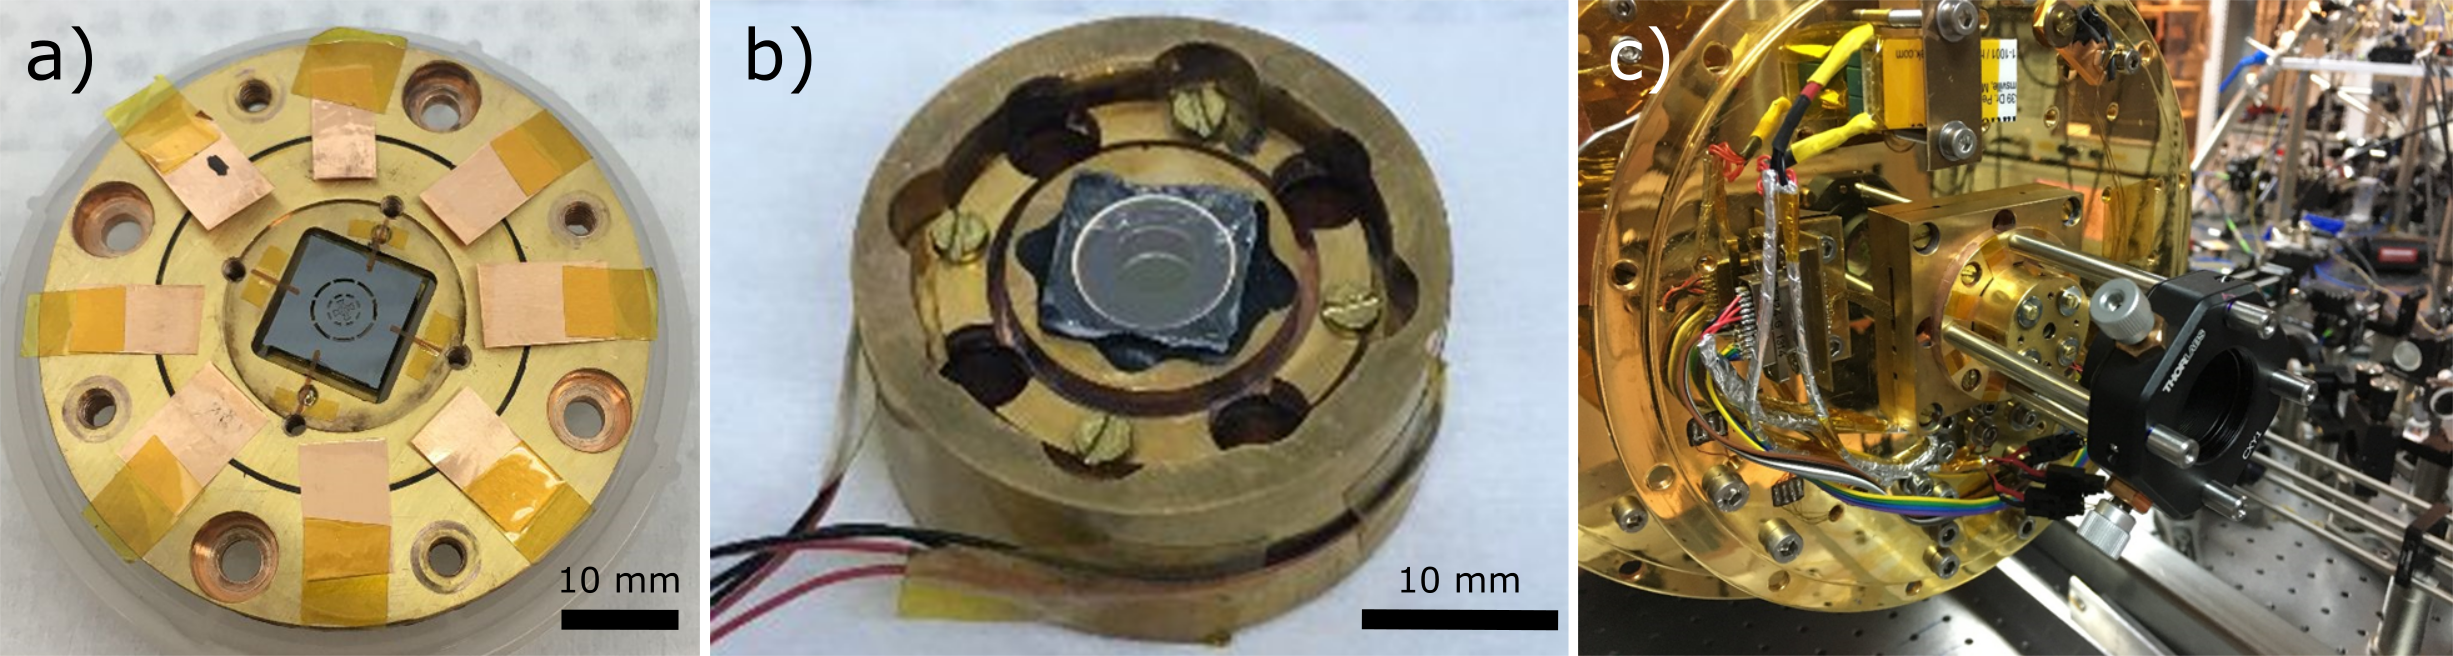
\includegraphics[height=129pt]{figures/optomechanical_cavity.png}
\caption{Cavité optomécanique formée par (a) l'oscillateur mécanique, ici un micro-disque, et (b) le miroir de couplage (\uroc).
Les câbles permettent de contrôler les cales piézoélectriques nécessaires à l'asservissement en longueur de la cavité.
La cavité assemblée (c) est montée sur le dernier étage du cryostat à dilution.
Une lentille de courte focale permet finalement d'adapter le faisceau incident au mode fondamental de la micro-cavité.}
\label{fig:cavity}
\end{figure}

\subsection{Couplage optomécanique et refroidissement}
\label{sec:optomechanics}

La températures à atteindre pour préparer un oscillateur mécanique dans son état quantique fondamental est de l'ordre de \unit{100}{\micro\kelvin} avec nos échantillons : $T_{Q,\mathrm{pilier}} = \unit{200}{\micro\kelvin}$ et $T_{Q,\mathrm{disque}} = \unit{10}{\micro\kelvin}$.
Il faut donc le refroidir de plus de six ordres de grandeur par rapport à la température ambiante.
L'ensemble de la cavité est donc refroidi dans un premier temps jusqu'à \unit{30}{\milli\kelvin} dans un cryostat à dilution fonctionnant avec un mélange $\mathrm{^4He/^3He}$.

\begin{mep}
L'obtention de telles températures présente un réel défi technologique : la conception des cryostats est soumise à de nombreuses contraintes liés notamment aux transferts thermiques.
En CPGE, le fonctionnement de ces machines thermiques peut être abordé en PC dans le cadre d'une approche thermodynamique simplifiée.
Il serait possible d'évaluer avec les étudiants l'importance de l'utilisation d'une enceinte sous vide, de matériaux de conductivités thermiques adaptées et d'accès optiques limitant le chauffage par rayonnement du corps noir.
\end{mep}

Les techniques propres à l'optomécanique en cavité\footnote{Aspelmeyer \textit{et al.}, Cavity Optomechanics, \textit{Rev. Mod. Phys.}, (2014)} permettent ensuite de refroidir l'oscillateur mécanique jusqu'aux températures requises.
Si le laser est légèrement désaccordée par rapport à la cavité, une perturbation de sa longueur provoquée par un déplacement du miroir mobile modifie la puissance intracavité, ce qui en retour change la force de pression de radiation exercée sur le miroir : c'est le \textit{couplage optomécanique}. 
En raison de la durée de vie finie des photons dans la cavité, l'ajustement de la puissance intracavité par rapport à une perturbation de longueur est retardé.
La modulation de la force de pression de radiation $F_\mathrm{rad}$ est donc déphasée par rapport aux déplacements du miroir et se décompose en deux termes :
\begin{itemize}
\item l'un en phase $\delta F_{\mathrm{rad}, x}$, dont le premier ordre est proportionnel au déplacement, est associé à une force de rappel qui s'ajoute au ressort mécanique et déplace simplement la pulsation propre $\Omega_m$ : c'est l'effet de \textit{ressort optique} ;
\item l'autre en quadrature $\delta F_{\mathrm{rad}, v}$, proportionnel à la vitesse du miroir, permet d'obtenir une force analogue à un frottement visqueux associé à un taux de dissipation $\Gamma_\mathrm{opt}$.
\end{itemize}
À la différence de la dissipation mécanique $\Gamma_m$ responsable du mouvement brownien, la dissipation optique $\Gamma_\mathrm{opt}$ se fait sans ajout de bruit thermique, ce qui permet de refroidir l'oscillateur : c'est la \textit{friction froide}.
Sa température effective $T_\mathrm{eff}$ est alors différente de celle de l'environnement $T_\mathrm{env}$ et on montre :
\begin{equation}
T_\mathrm{eff} = T_\mathrm{env} \frac{\Gamma_m}{\Gamma_\mathrm{eff}},
\end{equation}
où $\Gamma_\mathrm{eff} = \Gamma_m+\Gamma_\mathrm{opt}$.
Cette relation justifie l'utilisation d'oscillateurs avec des grands facteurs de qualité et l'utilisation d'un cryostat à dilution pour avoir $T_\mathrm{env}$ aussi faible que possible.
L'auto-refroidissement nécessite \og simplement \fg{} d'asservir la longueur de la cavité pour que $\omega_\mathrm{L} < \omega_\mathrm{cav}$, où $\omega_\mathrm{cav}$ est la pulsation de la cavité et $\omega_\mathrm{L}$ celle du laser\footnote{Si à l'inverse $\omega_\mathrm{L} > \omega_\mathrm{cav}$, $\delta F_{\mathrm{rad}, v}$ correspond à un terme d'amplification ($\Gamma_\mathrm{opt} < 0 $ et $T_\mathrm{eff} > T_\mathrm{env}$), pouvant mener à un système instable si $\Gamma_\mathrm{eff} < 0$.}.
Cette technique a permis d'atteindre un taux d'occupation de 20 phonons, limité par la puissance optique injectable dans la cavité.

\begin{figure}
\center
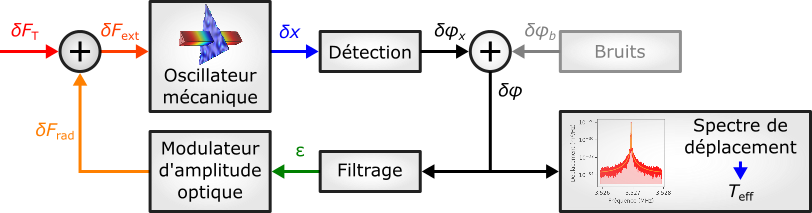
\includegraphics[scale=0.6]{figures/feedback_cooling_v2.png}
\caption{Principe du refroidissement par rétroaction.
La dissipation mécanique $\Gamma_m$ est responsable de la force de Langevin dont les fluctuations $\delta F_\mathrm{T}$ perturbent l'oscillateur.
La détection par interférométrie optique du déphasage $\delta \varphi_x$ associé au déplacement $\delta x$ donne accès à la température de l'oscillateur $T_\mathrm{eff}$ d'après le spectre de ses fluctuations de position.
Après filtrage, on obtient également un signal d'erreur $\epsilon$ qui permet de rétroagir sur l'échantillon par une correction adaptée de la force de pression de radiation $\delta F_\mathrm{rad}$ exercée par le faisceau incident.
La détection est imparfaite et l'ajout de bruit $\delta \varphi_b$ dégrade la sensibilité de mesure et diminue l'efficacité du refroidissement.}
\label{fig:feedback_scheme}
\end{figure}

En plus de la rétroaction passive inhérente au couplage optomécanique, on peut agir activement sur les déplacements du miroir mobile grâce au refroidissement par rétroaction (Fig.~\ref{fig:feedback_scheme}).
La mesure optique de la position de l'oscillateur sert à créer un signal d'erreur grâce auquel on applique une force de frottement visqueux sur le miroir mobile.
Le contrôle du déphasage introduit par la boucle de contrôle permet d'obtenir uniquement le terme de friction froide nécessaire au refroidissement.
La rétroaction peut être appliquée grâce à de nombreux actionneurs, mais dans notre expérience, on utilise un modulateur d'amplitude optique qui agit sur l'intensité du faisceau mesurant les déplacements de l'oscillateur.
La modulation d'amplitude ne perturbe pas la mesure puisqu'il s'agit d'une mesure de phase. 
À puissance optique égale, cette technique est plus efficace que l'auto-refroidissement puisque l'intensité de la rétroaction peut être facilement augmentée en accroissant le gain $g$ de la boucle de contrôle.

Dans le cas d'une mesure parfaite des déplacements du miroir, un accroissement du gain $g$ entraine toujours un refroidissement de l'oscillateur car seul le signal correspondant à ses déplacements est mesuré puis réinjecté dans la boucle.
Dans la réalité, la sensibilité est limitée par les fluctuations de position du miroir d'entrée, le bruit électronique et ultimement, les bruits quantiques.
Il existe donc un gain optimal $g_\mathrm{opt}$ pour lequel le mouvement brownien de l'oscillateur est équivalent au bruit de la mesure.
Pour $g>g_\mathrm{opt}$, le bruit de la mesure perturbe la rétroaction et sa contribution à l'agitation de l'oscillateur provoque une élévation de la température effective : le refroidissement est maximal pour $g=g_\mathrm{opt}$.
La sensibilité des mesures de déplacement est donc l'enjeu majeur pour atteindre l'état quantique fondamental.

\subsection{Contrôle de l'expérience : Arduino, RedPitaya et Python}
\label{sec:controls}

L'expérience dépend de plusieurs filtres et amplificateurs analogiques et numériques.
J'ai donc notamment réalisé des filtres électroniques passifs et actifs, des photodiodes à haute efficacité quantique et faible bruit et un contrôleur fondé sur une carte Arduino interfacé avec Python permettant le positionnement reproductible d'une translation motorisée.

Le bon fonctionnement du système repose également sur de nombreuses boucles de rétroaction en plus de celle utilisée pour le refroidissement : stabilisations de températures, de puissances optiques et asservissement de longueur portant sur la position des miroirs des cavités et interféromètres.
Excepté le refroidissement par rétroaction analogique, ces asservissements sont réalisés numériquement par des micro-contrôleurs RedPitaya et la bibliothèque PyRPL\footnote{\url{https://pyrpl.readthedocs.io/en/latest/}} (Python RedPitaya Lockbox) développée au sein de l'équipe.
Il est ainsi possible de piloter une grande partie de l'expérience à partir d'un PC, ce qui permet l'automatisation des séquences de mesures grâce à un répertoire de scripts Python que j'ai pu étoffer.

\begin{mep}
Ces systèmes bouclés m'ont permis de développer une compréhension par l'expérience des systèmes asservis, renforcée par la suite par une approche plus théorique.
Ceci me sera utile pour aborder ce thème avec des étudiants en PSI.
Les compétences que j'ai acquises dans la programmation, l'électronique analogique et numérique et dans l'utilisation de micro-contrôleurs permettrons d'illustrer mes cours de simulations, mais aussi de guider mes élèves dans le cadre de l'enseignement scientifique.
Les cartes RedPitaya ($\sim\unit{200}{\text{\euro}}$) disposent nativement d'un oscilloscope et d'une GBF numérique.
L'utilisation du programme \textit{open source} PyRPL ouvre par ailleurs de nombreuses perspectives :  analyseur de spectre et de réseau ou boite d'asservissement pour ne citer que les fonctionnalités déjà implémentées.
Cette ressource pourrait être introduite comme évolution de l'Arduino à des élèves de lycée et exploitée dans le cadre de travaux pratiques en CPGE.
\end{mep}

\subsection{Principaux résultats obtenus}
\label{sec:results}

Après avoir caractérisé les échantillons mécaniques et réalisé les micro-miroirs de couplage, la cavité optomécanique est alignée et montée dans le cryostat à dilution puis refroidie vers \unit{30}{\milli\kelvin}.
Sa longueur moyenne est asservie sur le laser et on optimise les paramètres de la boucle de contrôle du refroidissement par rétroaction.
Cette phase s'accompagne d'une identification méticuleuse des parasites électroniques, acoustiques et optiques qui compromettent la stabilité de l'expérience pour les atténuer.
On acquiert finalement le spectre des fluctuations de position de l'oscillateur en faisant varier le gain $g$ du refroidissement par rétroaction avec des atténuateurs analogiques.
Les résultats obtenus avec un micro-pilier sont visibles sur la Fig.~\ref{fig:feedback_cooling_pillar}.

Il a ainsi été possible de refroidir le micro-pilier jusqu'à une température effective $T_\mathrm{eff} = \unit{1{,}0\pm 0{,}1}{\milli\kelvin}$, ce qui correspond à un taux d'occupation de $\mathbf{5{,}3 \pm 0{,}5}$ \textbf{phonons}.
Des limitations importantes principalement attribuées à la dégradation progressive de l'échantillon, conduisant notamment à des instabilités photothermiques nous ont conduit à utiliser l'autre type d'oscillateur : les micro-disques.
Avec ces échantillons et en seulement quelques mois, il a été possible d'atteindre une température de \unit{0{,}7\pm 0{,}1}{\milli\kelvin} correspondant à un niveau d'occupation de $\mathbf{55\pm5}$ \textbf{phonons}, cette fois limité par le bruit de détection causé par les fluctuations de position du miroir d'entrée de la cavité.
À température comparable, le niveau d'occupation de l'oscillateur obtenu avec le micro-disque est dix fois plus élevé que celui du micro-pilier car la fréquence du mode propre des micro-disques est dix fois plus faible ($T_Q = \hbar\Omega_m/k_B$).
Ces résultats font état des \textit{taux d'occupation thermique les plus faibles atteints actuellement avec des oscillateurs mécaniques aussi macroscopiques} ($m_\mathrm{eff}\approx\unit{100}{\micro\gram}$). 

\begin{figure}
\center
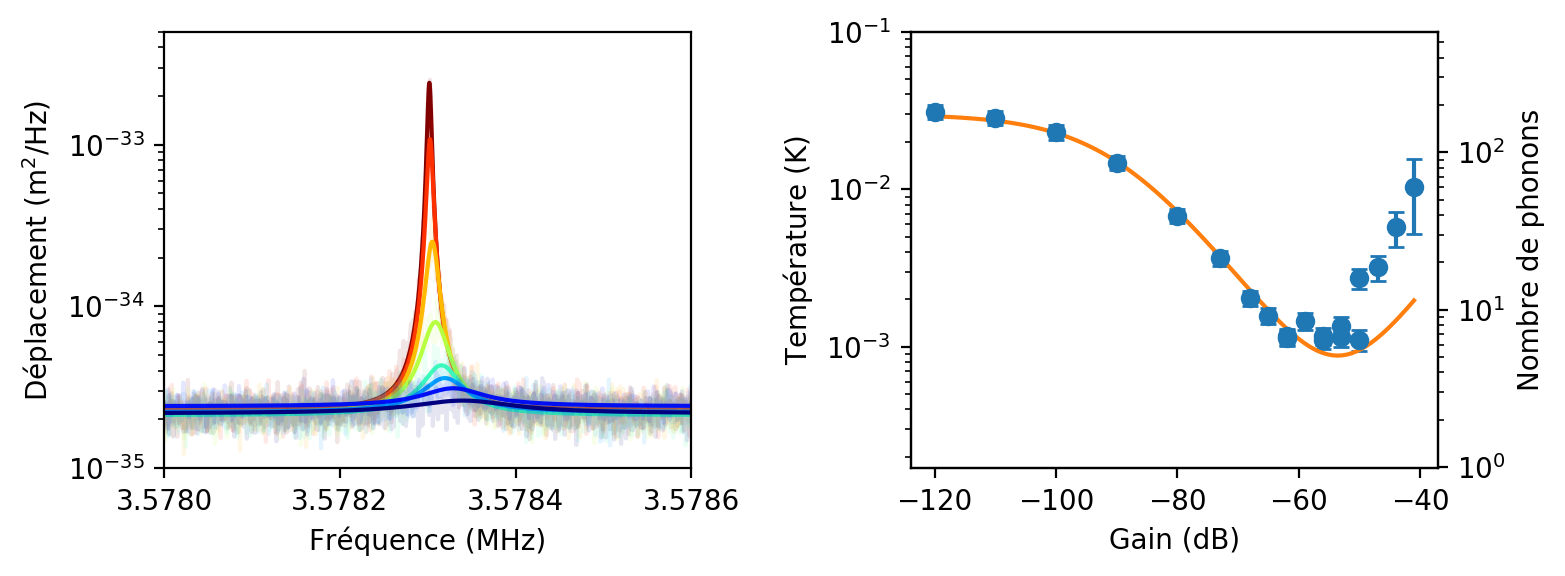
\includegraphics[scale=0.75]{figures/feedback_cooling_6phonons.png}
\caption{Refroidissement d'un micro-pilier proche de son état quantique fondamental.
À gauche : spectres des fluctuations de position obtenus pour différents gains (du rouge pour les gains faibles au violet pour le gain optimal).
Les données expérimentales sont tracées en transparence et l'ajustement lorentzien par le modèle théorique correspond aux courbes pleines.
À droite : températures effectives $T_\mathrm{eff}$ déduites de l'intégrale des courbes précédentes.
La courbe orange correspond au modèle qui tient compte des paramètres de l'expérience.}
\label{fig:feedback_cooling_pillar}
\end{figure}

\subsection{Vers des mesures sous la limite quantique standard}
\label{sec:prospects}

Dans notre expérience, le signal que l'on mesure est associé au mouvement brownien de l'oscillateur, concentré autour de la pulsation mécanique $\Omega_m$.
La limite de sensibilité de la plupart de nos mesure est imposé par le bruit quantique de phase, qui forme le plancher observé vers $\unit{2\times10^{-35}}{\meter\squared{.}\hertz^{-1}}$ sur la Fig.~\ref{fig:feedback_cooling_pillar}.
Compte tenu des puissances optiques utilisées et du niveau d'occupation thermique atteint, le bruit quantique d'intensité ne représente qu'une fraction de l'ordre de \unit{1}{\%} des fluctuations de position mesurées.
Grâce aux développements réalisés sur la cavité optomécanique, une observation du bruit de pression de radiation devrait être possible, notamment en utilisant une puissance optique plus importante puisque l'amplitude de ce bruit est proportionnel à l'amplitude du rayonnement lumineux.
Même si l'origine du signal est complètement différente, il sera alors possible de réaliser des mesures de déplacements limitées par les mêmes bruits quantiques que les interféromètres gravitationnels.

En remplaçant le laser actuel par une source de lumière comprimée, on obtient un état de la lumière dont les fluctuations de phase, d'intensité ou d'une combinaison des deux sont plus faibles que celles d'un état cohérent.
L'inégalité d'Heisenberg interdit cependant une réduction simultanée des fluctuations de phase et d'intensité.
En exploitant la dépendance du déphasage introduit par une cavité optique avec la fréquence, on obtient une réduction du bruit d'intensité à la fréquence de résonance de l'oscillateur où la réponse mécanique du système à la pression de radiation est maximale,  et une réduction du bruit de phase loin de la résonance.
Cette technique est actuellement développée dans l'équipe et permettra des mesures sous la limite quantique standard.
Elle sera ensuite implémentée sur Virgo lors des prochaines campagnes de mesure afin d'étendre la portée du détecteur et ainsi observer plus d'évènements
Augmenter la sensibilité de l'appareil par un facteur deux double sa porté, ce qui multiplie par huit le volume d'univers observable et donc la probabilité d'observer des sources d'ondes gravitationnelles.

\section{Enseignement, diffusion et vulgarisation}

\subsection{Enseignements}

Au cours de ma thèse, j'ai pu effectuer une mission d'enseignement qui m'a donné l'occasion de mettre en pratique plusieurs approches de l'enseignement.
L'unité d'enseignement de physique expérimentale est certainement celle qui m'a le plus apporté.
Cette UE ne contient aucun cours magistral et se compose d'une série de TP abordant l'électronique numérique et analogique ainsi que la programmation (Labview).
Chaque séance de TP est précédée d'un TD dont l'objectif est surtout de présenter aux étudiants le matériel qu'ils devront utiliser et d'aborder par l'expérience les concepts nouveaux.
Les TP les confrontent ensuite à des objectifs concrets, comme la réalisation d'un bras capable de détecter et saisir un objet, où ils doivent exploiter et se familiariser avec ces nouveaux concepts.
Ils disposent enfin d'une grande liberté pour l'objectif de fin de semestre, une compétition de robots dont les règles varient : combats de \og sumos\fg{}, positionner un drapeau au plus près d'une cible, etc.

Le parcours des étudiants que j'ai pu encadrer est souvent très disparate et il m'a parfois été difficile de m'adapter à chacun.
Leur investissement était toutefois réel et les séances très interactives.
Cette approche par l'expérience me semble essentielle puisqu'elle amène les étudiants à se poser eux-même les questions grâce auxquelles ils apprennent des notions nouvelles.
La nature même de ma thèse, profondément expérimentale, renforce cette conviction puisqu'elle m'a permis d'acquérir de nombreuses compétences et de consolider mes connaissances théoriques dans plusieurs domaines.
C'est une méthode d'enseignement très vivante dont je ne manquerai pas de m'inspirer en tant qu'enseignant.

\subsection{Vulgarisation : résonance et ondes gravitationnelles}

Le sujet et le contexte de ma thèse m'ont amené à plusieurs reprises à des activités de médiation auprès de publics très variés.
L'actualité récente depuis fin 2015 autour des ondes gravitationnelles a permis de mettre en avant tous les travaux liés à leur détections et à l'implication de telles observations.
J'ai ainsi pu réaliser des présentations la détection des ondes gravitationnelles devant des lycéens à l'occasion des Olympiades de physique, des fêtes de la Science organisées à Jussieu (Sorbonne Université), devant le personnel technique et administratif du LKB et finalement au Palais de la Découverte pour l'exposition \textit{Un chercheur, Une manip}.
La préparation, la présentation et les échanges qui ont suivi ces présentations ont été autant d'occasion de s'approprier différents aspects liés à ce thème, mais aussi d'expérimenter différentes approches afin de faire passer au mieux mon message.
Ce sujet, par la variété des domaines qu'il fait intervenir, peut servir de fil conducteur et permette de rattacher les sujets abordés en cours à une actualité scientifique qui promet de nombreux rebondissements.
On peut, sans exhaustivité, aborder les systèmes à deux points, l'oscillateur harmonique, l'interférométrie, les asservissements, le traitement du signal, etc.
La communauté LIGO/Virgo est très dynamique et offre des ressources qu'il est possible de réinvestir à tous les niveaux : articles\footnote{Mathur \textit{et al.}, An Analysis of the LIGO Discovery based on Introductory Physics, \textit{Am. J. Phys.}, (2017)}, données, etc.

À l'occasion du sujet \textit{Peut on casser un verre avec la voix ?} de l'émission E=M6, j'ai aussi mis en place une expérience permettant de casser un verre en le faisant vibrer à l'aide d'un haut-parleur.
%\footnote{\url{https://youtu.be/7cgZcbHmxm4}}
Après avoir réalisé des simulations par éléments finis (Fig.~\ref{fig:wine_glass}), on peut observer expérimentalement les différents modes propres d'un verre et visualiser les vibrations à l'aide d'un stroboscope.
Cette expérience permet notamment d'aborder l'analyse spectrale et le phénomène de résonance, et pourrait faire l'objet d'une manipulation de TP (un peu bruyante certes) sans aller nécessairement jusqu'à la rupture.

\begin{figure}
\center
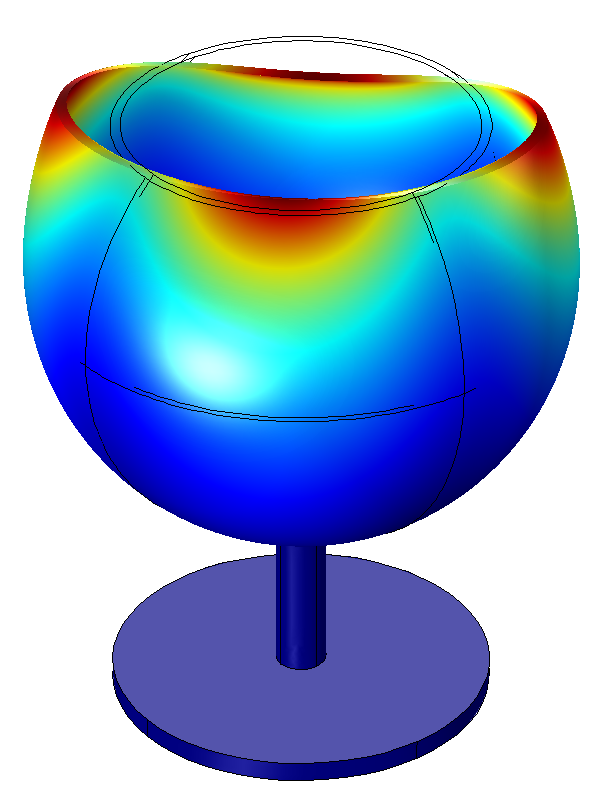
\includegraphics[height=100pt]{figures/wine_glass_f0.png}
\hfill
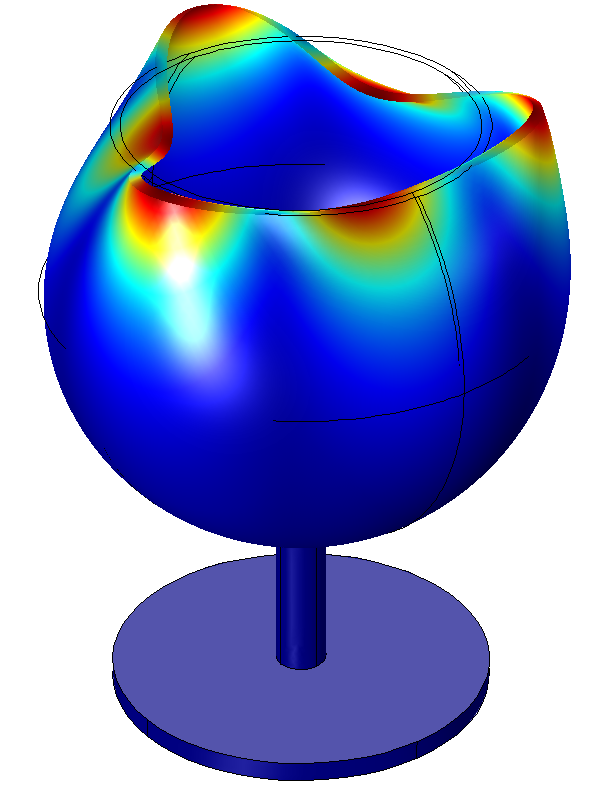
\includegraphics[height=100pt]{figures/wine_glass_f1.png}
\hfill
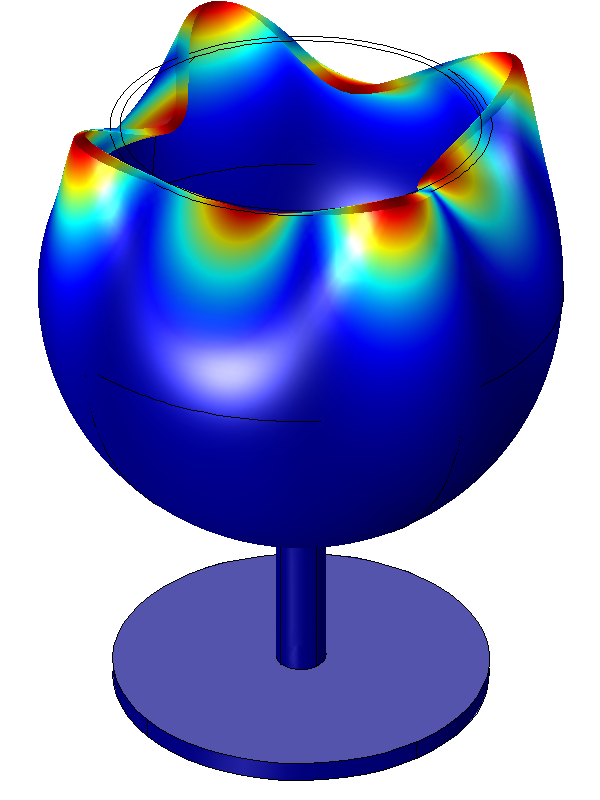
\includegraphics[height=100pt]{figures/wine_glass_f2.png}
\hfill
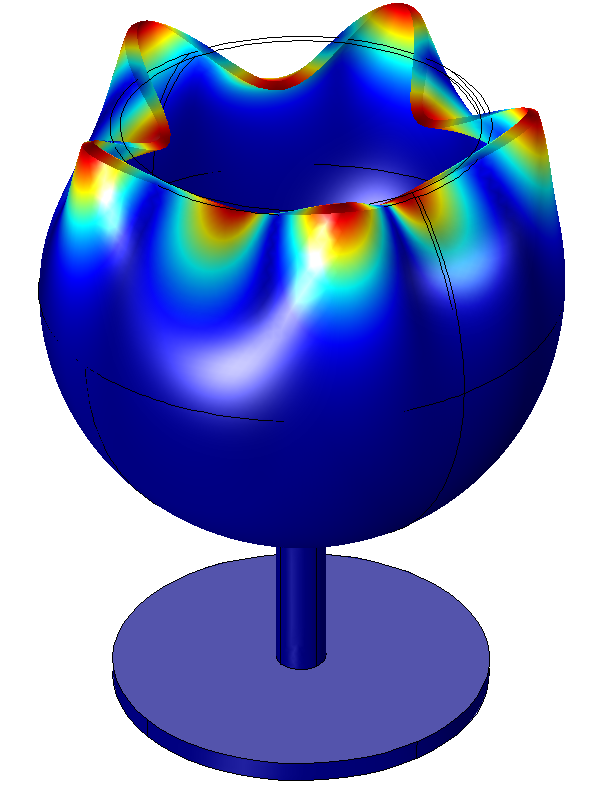
\includegraphics[height=100pt]{figures/wine_glass_f3.png}
\hfill
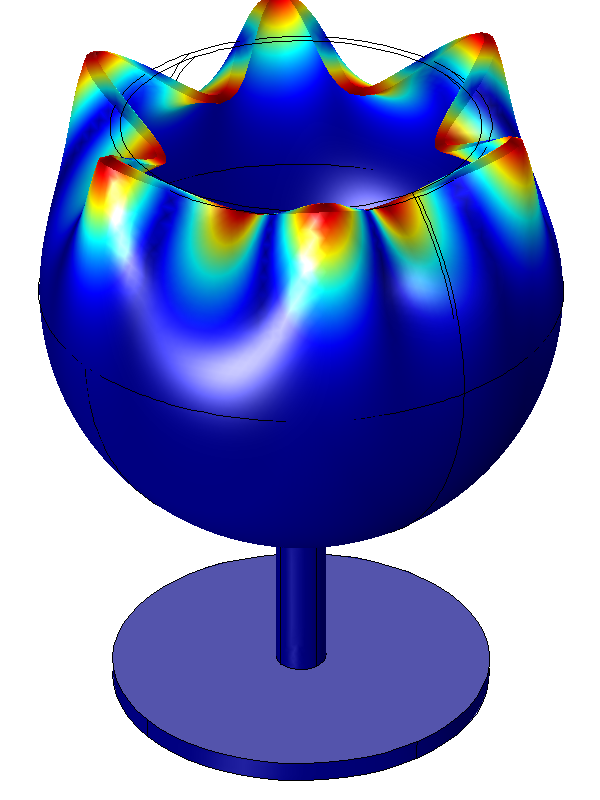
\includegraphics[height=100pt]{figures/wine_glass_f4.png}
\caption{Simulations par élément fini (COMSOL) des premiers modes de vibration d'un verre.}
\label{fig:wine_glass}
\end{figure}

\end{document}